
\documentclass{beamer}

%\usetheme{Hannover}
%\usecolortheme{seahorse}

\usecolortheme{whale}

%\usecolortheme{beaver}
%\usecolortheme{orchid}

%\usecolortheme{crane}
%\useoutertheme{smoothbars}
\useinnertheme[shadow=false]{rounded}
\useoutertheme[footline=authortitle]{miniframes}

\usebackgroundtemplate%
{%		
	\hspace*{-0.3cm}
	
\includegraphics[width=0.5\paperwidth]{logo_ins.png}
	\hspace*{5cm}
	
\includegraphics[width=5.5\paperwidth]{logo_ins.png}
}

\usepackage{multimedia}

\usepackage[utf8]{inputenc}
\usepackage[T1]{fontenc}

\usepackage{multimedia}
\usepackage{amssymb}
\usepackage{amsmath}
%\usepackage[francais]{babel}

\setbeamertemplate{footline}[text line]{%
	\parbox{\linewidth}{ \vspace*{-15pt}
		\hspace{3cm}
		\insertshortauthor 
		\hfill %\hspace*{2cm} 
		IJCNN 2015 \hfill \insertpagenumber}}

% Avec cette commande, le plan sera rappel? 
% ? chaque changement de section
\AtBeginSection[]{
  \frame<handout:0>{
    \frametitle{Plan}
    \tableofcontents[current]
  }
}

\title[Fast classifier adaptation in non-stationary environments]
{Reward-based online learning in non-stationary environments: 
	Adapting a P300-speller with a ``Backspace'' key}


%\author[Daucé et al.]{author1 \inst{1} \and author2 \inst{2}}

                      
\author[Daucé et al.]{Emmanuel Daucé \inst{1} \inst{2} \and Timothée Proix \inst{2} \and Liva Ralaivola \inst{3}}

\institute[Centrale Marseille / Aix-Marseille Université]{\inst{1} Ecole Centrale Marseille \and %
                      \inst{2} INS - Aix-Marseille Université - Inserm UMR 1106 \and %
                      \inst{3} LIF - Aix-Marseille Université - CNRS UMR 7229}

\begin{document}

\begin{frame}\titlepage
\end{frame}

\begin{frame}\frametitle{Table of contents}
  \tableofcontents
\end{frame}

\section{Introduction}
\subsection*{}

\begin{frame}\frametitle{Brain-Computer Interfaces}
	\vspace{-.8cm}
		\begin{itemize}
		\item Embedded classifiers:
		\begin{itemize}
			\item real-time
			\item noisy (EEG)
			\item subject/use case specific
			\item non-stationary 
		\end{itemize}
		$\Rightarrow$ Adaptive Learning  
		\item Brain Computer Interfaces, a tool for :
		\begin{itemize}
			\item Communication (in the absence of a motor capabilities) 
			\item Brain monitoring / neurofeedback
			\item Motor rehabilitation
		\end{itemize}
		\item ``CO-ADAPT'' project : INRIA Sophia/ INSERM Lyon/ CNRS LATP, ... (French ANR funding)
		\begin{itemize}
			\item ``co-adaptive'' motor imagery
			\item ``co-adaptive'' P300 speller
		\end{itemize}
	\end{itemize}
\end{frame}




%%%%%%%%%%%%%%%%%%%%%%%%%%%%%%%%%%%%%%%%%%%%%%%%%%%%%%%%%%%%
\begin{frame}\frametitle{Embedded classifiers}
	\vspace{-1cm}
	\begin{itemize}
		\item Classification problem : sources $\rightarrow$ signal $\rightarrow$ features extraction $\rightarrow$ classification
		\begin{itemize}
			\item adaptive feature extraction
			\item adaptive classification
		\end{itemize}
		\item Online learning : ``light'' classifier update at each processing step
		\begin{itemize}
			\item supervised online learning: stochastic gradient descent
			\item unsupervised online learning: online mobile centers (K-means, EM,...) 
			\item reward-based online learning: stochastic classifiers + policy/value iteration 
			\begin{itemize}
				\item exploration/exploitation trade-off
				\item which reward?
			\end{itemize}
		\end{itemize}
	\end{itemize}
\end{frame}


\begin{frame} \frametitle{P300 speller}
	\vspace{-.8cm}
	\begin{itemize}
		\item EEG : 
	\vspace{-.1cm}		
		\begin{itemize}
			\item 10 - 60 channels (surface electric potential - H Berger, 1929)
			\item high temporal resolution / low spatial resolution
			\item noisy, non-reliable,... ``Evoqued potentials'' technique
			\item the ``P300'' ERP is ``surprise'' effect (``oddball'' paradigm)
		\end{itemize}
	\end{itemize}
	\vspace{-.3cm}
	\begin{columns}
		\begin{column}{0.75\linewidth}
			\begin{itemize}
				\item P300-speller (Farwell and Donchin, 1988):
				\begin{itemize}
					\item based on the ``oddball'' paradigm
					\item 6 x 6 letters grid
					\item random row/column magnification (every 150-300 ms)
					\item row/column evidence build-up + argmax choice
					\item low SNR / low bit rate (many flashes for one letter)
					\item spelling accuracy tends to decrease in the long run
				\end{itemize}
			\end{itemize}
		\end{column}
		\begin{column}{0.25\linewidth}
			\centerline{
				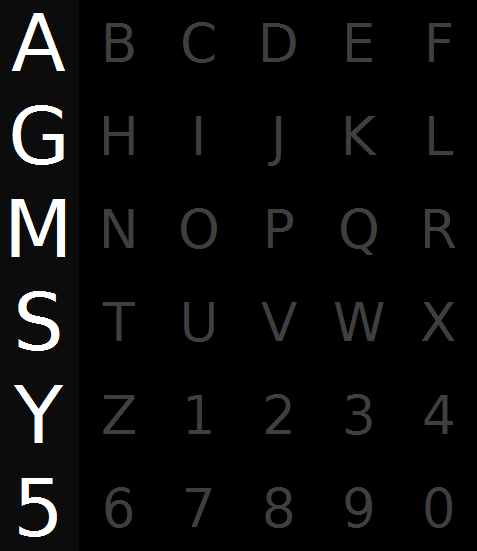
\includegraphics[width=\linewidth]{P300_grid.png}
			}
		\end{column}
	\end{columns}
\end{frame}

\begin{frame}\frametitle{EEG data (from Inserm U1028, Lyon, France)}
	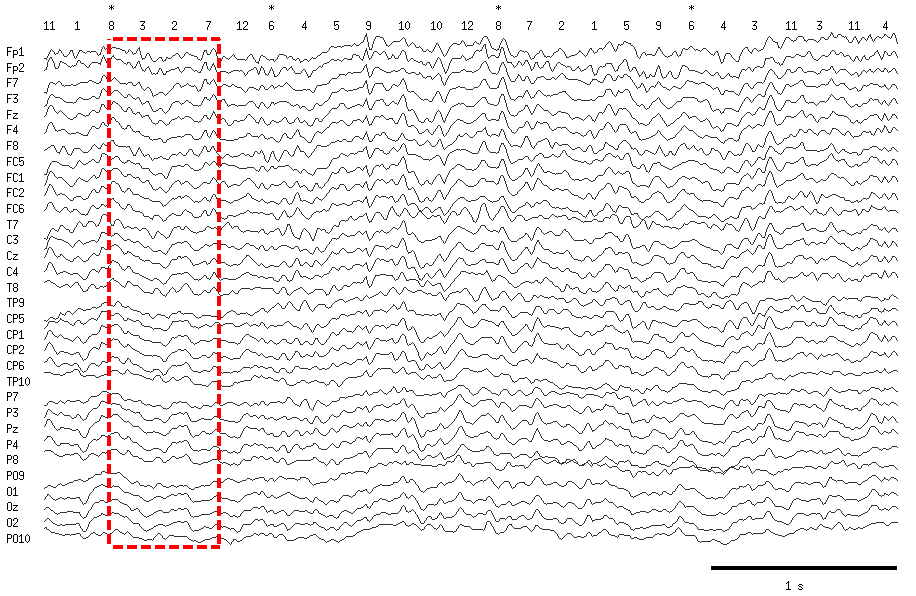
\includegraphics[width=\linewidth]{EEG.png}
\end{frame}

\begin{frame}\frametitle{Data processing pipeline}
	\vspace{-1cm}
	\centerline{
		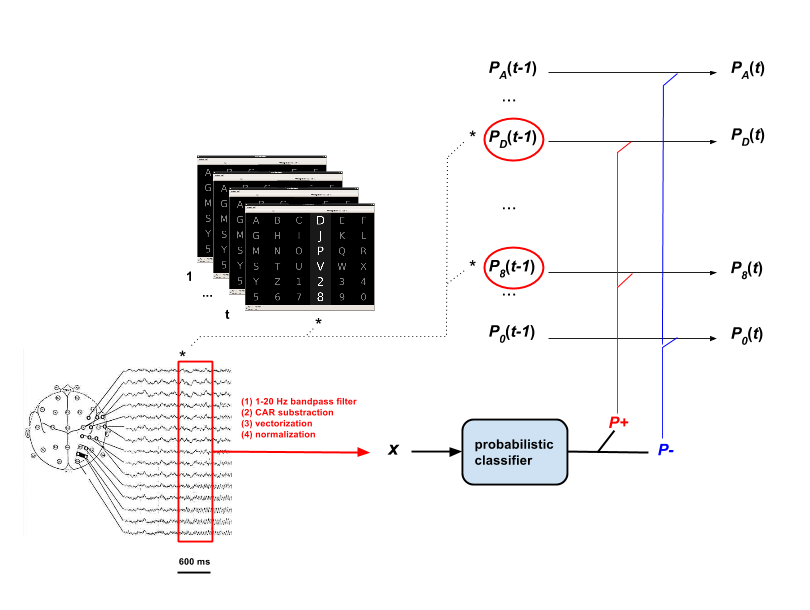
\includegraphics[width=.9\linewidth]{overview.png}
	}
\end{frame}

\begin{frame}\frametitle{P300-speller roadmap}
	\vspace{-.5cm}
	\begin{itemize}
		\item Transfer learning \footnotesize{\cite{Kindermans12b, Congedo13}}: 
		\vspace{-.1cm}
		\begin{itemize}
			\item Across subjects 
			\item generic classifier ``pre-learning''
			\item smart initialization
		\end{itemize}
		\item Optimal display
		\item Evidence build-up \footnotesize{\cite{Perrin12,Kindermans2013}}:
		\vspace{-.1cm}
		\begin{itemize}
			\item Probabilistic classifier : posterior estimate
			\item Evidence accumulation
			\item Threshold-based dynamic stopping
			\item Speed-accuracy trade-off
		\end{itemize}
		\item Online learning : 
		\vspace{-.1cm}
		\begin{itemize}
			\item Toward a subject-specific classifier
			\item Recover from unexpected changes
			\item Different approaches :
			\begin{itemize}
				\item EM \footnotesize{\cite{Li06,Kindermans12}}
				\item RL \footnotesize{\cite{Dauce2013}}
			\end{itemize}
		\end{itemize}  
	\end{itemize}
	
\end{frame}
%\section{Oddball classification}
%\subsection*{}
%
%\begin{frame} \frametitle{P300 speller}
%\begin{itemize}
%  \item EEG : 
%  \begin{itemize}
%    \item 10 - 60 channels (surface electric potential - H Berger, 1929)
%    \item high temporal resolution / low spatial resolution
%    \item noisy, non-reliable,... ``Evoqued potentials'' technique
%    \item the ``P300'' ERP is ``surprise'' effect (``oddball'' paradigm)
%  \end{itemize}
%\end{itemize}
%\begin{columns}
% \begin{column}{0.75\linewidth}
%\begin{itemize}
%  \item P300-speller (Farwell and Donchin, 1988):
%    \begin{itemize}
%      \item based on the ``oddball'' paradigm
%      \item 6 x 6 letters grid
%      \item random row/column magnification (every 150-300 ms)
%      \item row/column evidence build-up + argmax choice
%      \item low SNR / low bit rate (many flashes for one letter)
%      \item spelling accuracy tends to decrease in the long run
%    \end{itemize}
%\end{itemize}
%\end{column}
%\begin{column}{0.25\linewidth}
% \centerline{
% 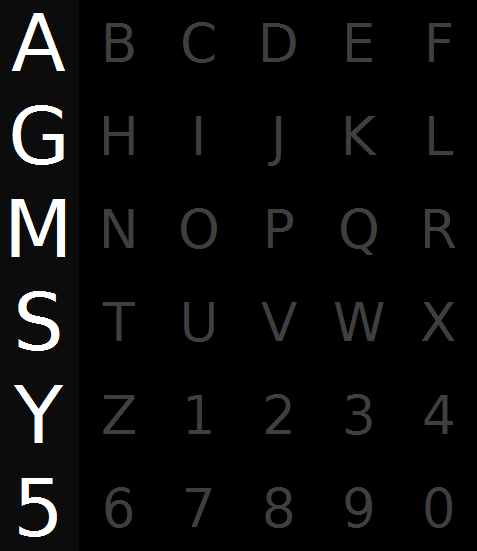
\includegraphics[width=\linewidth]{P300_grid.png}
% }
%\end{column}
%\end{columns}
%\end{frame}
%
%\begin{frame}\frametitle{EEG data (from Inserm U1028, Lyon, France)}
% 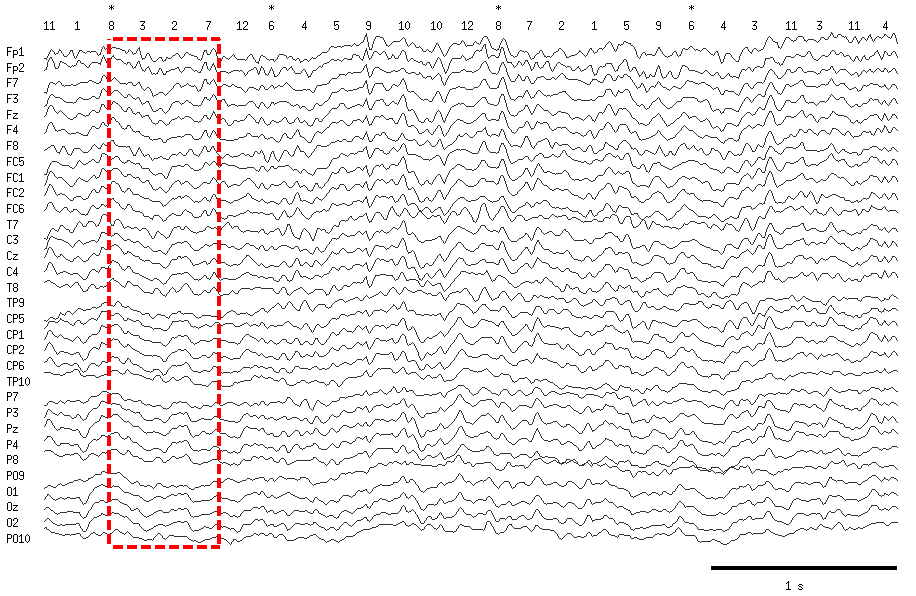
\includegraphics[width=1\linewidth]{EEG.png}
%\end{frame}
%
%
%\begin{frame}\frametitle{The ``oddball'' classification problem}
%\begin{columns} 
% \begin{column}{0.5\linewidth}
% 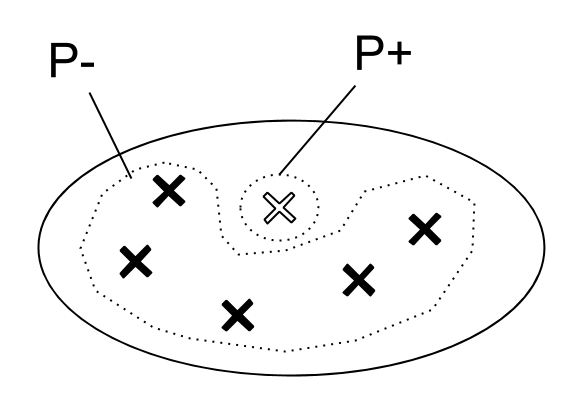
\includegraphics[width=\linewidth]{oddball_s.png}
% \end{column}
% \begin{column}{0.5\linewidth}
%  \begin{itemize}
%   \item Set of $K$ observations
%   \item one vs. ``the rest'' classification 
%  \end{itemize}
% \end{column}
%
%\end{columns}
%\begin{align}
% P(k|x_1,...,x_K) &=  \frac{P(x_1,...,x_K,k)}{P(x_1,...,x_K)}\nonumber\\
%                  &= \frac{                 P^+(x_k)          \Pi_{\ell \neq k}        P^-(x_\ell)         }
%                          { \sum_{k^\prime} P^+(x_{k^\prime}) \Pi_{\ell^\prime \neq k^\prime} P^-(x_{\ell^\prime})} \nonumber
%                  &= \frac{\frac{P+(\boldsymbol{x}_k)}{P^-(\boldsymbol{x}_k)}}
%                                          {\sum_{\ell} \frac{P^+(\boldsymbol{x}_\ell)}{P^-(\boldsymbol{x}_\ell)}}      
%\end{align}
%
%\end{frame}
%
%
%
%\begin{frame}  \frametitle{The ``oddball'' classification and probabilistic classifiers :}
%  \begin{itemize}
%  \item The oddball classification problem is ``in between'' binary and multiclass problems. 
%  \begin{footnotesize}
%    \begin{tabular}{|c||c|c|}
%      \hline
%      & {\bf Model-based} & {\bf Model-free (Softmax-linear)} \\
%      \hline\hline
%      Binary  & 
%      $P(1|\boldsymbol{x}) = \frac{1}{1 + \frac{P^-(\boldsymbol{x})}{P^+(\boldsymbol{x})}}$ &
%      $\pi(\boldsymbol{x};\boldsymbol{w}, b) = \frac{1}{1 + exp(- \boldsymbol{x} \boldsymbol{w}^T + b)}$\\
%      \hline
%      ``Oddball''  & 
%      $P(k|\boldsymbol{x}_1,...,\boldsymbol{x}_K) = \frac{\frac{P^+(\boldsymbol{x}_k)}{P^-(\boldsymbol{x}_k)}}
%                                          {\sum_{\ell} \frac{P^+(\boldsymbol{x}_\ell)}{P^-(\boldsymbol{x}_\ell)}}$ &
%                                     
%      $\pi_k(\boldsymbol{x}_1,...,\boldsymbol{x}_K;\boldsymbol{w}) =  \frac{\exp(\boldsymbol{x}_k \boldsymbol{w}^T)}
%                                             {\sum_\ell  \exp(\boldsymbol{x}_\ell \boldsymbol{w}^T)}$\\
%      \hline
%      Multiclass  &
%      $P(k|\boldsymbol{x}) = \frac{P(\boldsymbol{x}|k)} {\sum_\ell P(\boldsymbol{x}|\ell)}$  &
%      $\pi_k(\boldsymbol{x}; \boldsymbol{w}_1, ..., \boldsymbol{w}_K) = \frac{\exp(\boldsymbol{x} \boldsymbol{w}_k^T)}{\sum_\ell \exp(\boldsymbol{x} \boldsymbol{w}_\ell^T)}$\\
%      \hline
%    \end{tabular}  
%  \end{footnotesize}
%  \item The ``objective'' $\boldsymbol{w}$ is $(\boldsymbol{\mu}^+ - \boldsymbol{\mu}^-)\Sigma^{-1}$ (Multivariate Homoscedastic Gaussian model)
%  \end{itemize}
%\end{frame}

\section{Reward-based learning}
\subsection*{}

\begin{frame} \frametitle{Reinforcement learning : multiple approaches}
	\vspace{-.6cm}
  \begin{itemize}
    \item general RL problem :
    \vspace{-.1cm}
    \begin{itemize}
      \item observations : $x_1$, ..., $x_T$
      \item policy (random decision = exploration) : $\pi(x,y) = P(y|x)$
      \item responses : $y_1$, ..., $y_T$
      \item reward : $r_T \in \mathbb{R}$ 	
    \end{itemize}
    \item Task : try to improve the politics for increasing time/trial
        \vspace{-.1cm}
    \begin{itemize}
      \item Actor-critic / Q-learning :
          \vspace{-.1cm} 
      \begin{itemize}
       \item temporal credit assignment (delayed reward)
       \item discrete state/action space (LUT)
       \item Value update vs. action 
      \end{itemize}
      \item Multi-armed bandit : 
          \vspace{-.1cm}
      \begin{itemize}
        \item instant reward
        \item contextual bandit
      \end{itemize}  
      \item Policy-gradient : 
          \vspace{-.1cm}
      \begin{itemize}
        \item instant or delayed rewards
        \item discrete or continuous state/actions space
        \item direct update of the policy
      \end{itemize}  
    \end{itemize}
    %\item The policy gradient approach: 
    %\begin{itemize}
    %  \item Direct improvement of the policy $\pi_\mathbf{w}$
    %  \item by changing the set of parameters with the policy gradient estimate $\hat{E}(\nabla_\mathbf{w}r\ln\pi_\mathbf{w}(x,y))$ (Williams, 1992)
    %\end{itemize}
  \end{itemize}
\end{frame}

\begin{frame}{Rewards in classifiction}
	\vspace{-1cm}
 \begin{itemize}
  \item Optimal $\boldsymbol{w}$ unknown $\rightarrow$ model-free, trial and error
  \item Online stochastic classifier :
  \begin{itemize}
    \item read input observations set : $\underline{\mathbf{x}} = (\boldsymbol{x}_1,...,\boldsymbol{x}_K)$
    \item give a score to every class : $\forall k, \pi(\underline{\mathbf{x}},k;\boldsymbol{w}) =  \frac{\exp(\boldsymbol{x}_k \boldsymbol{w}^T)}
                                             {\sum_{l}  \exp(\boldsymbol{x}_l \boldsymbol{w}^T)}$ 
    \item choose the response at random (Softmax choice)
    \item read the \emph{reward} $r$
    \item update $\boldsymbol{w}$
  \end{itemize}
  \item Which reward ?
  \begin{itemize}
    \item ``error'' potential after the classifier's response:
 \centerline{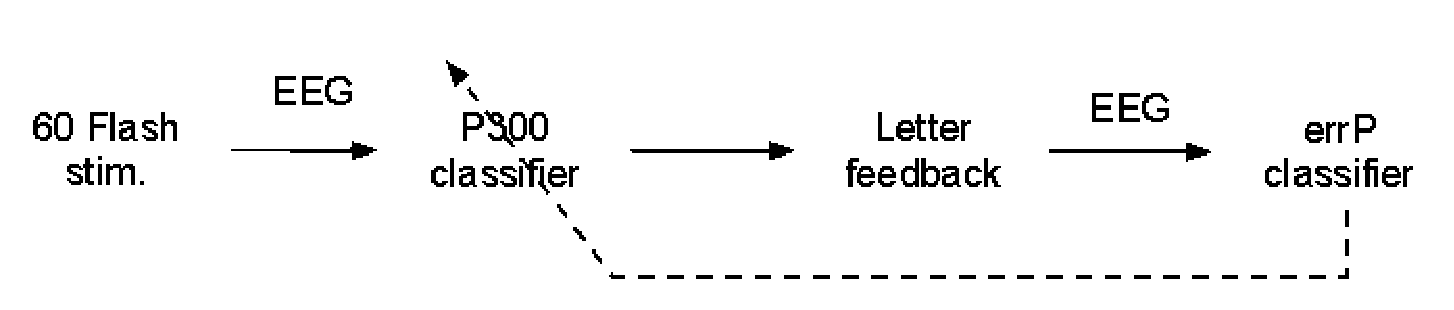
\includegraphics[width=0.7\linewidth]{online_P300.pdf}}
    \item ``BACKSPACE'' key on the virtual keyboard
  \end{itemize}
 \end{itemize}
\end{frame}

\begin{frame}\frametitle{Learning and forgetting : Regularized Policy gradient update}
	\vspace{-.8cm}
 \begin{itemize}
  \item Regularized optimization ($\lambda$ hyperparameter):
  \vspace{-.4cm} 
  $$\max _{\boldsymbol{w}} \mathcal{H} = \max _{\boldsymbol{w}} E(r) - \frac{\lambda}{2}||\boldsymbol{w}||^2$$
  \vspace{-.4cm}
  \item Regularized gradient ascent : 
  \footnotesize{$\nabla_w \mathcal{H} = {E}({\color{blue}r\nabla_\mathbf{w}\ln\pi(\underline{\mathbf{x}},y;\mathbf{w})}) - \lambda \boldsymbol{w}$ }
  \begin{itemize}
    \item Gradient estimator (stochastic gradient) :
    \vspace{-.2cm} 
    $$
    % E(  r \nabla_\mathbf{w}\ln\pi(\underline{\mathbf{x}},y,\mathbf{w}) ) 
     %  \simeq 
       \langle {\color{blue}r_t \nabla_\mathbf{w}\ln\pi(\underline{\mathbf{x}}_t,y_t;\mathbf{w})}\rangle_{1..T} $$
    \item Online update (learning rate $\eta << 1$):
        \vspace{-.2cm} 
    \begin{align}
      \boldsymbol{w} &\leftarrow \boldsymbol{w} + \eta ( {\color{blue}r \nabla_\mathbf{w}\ln\pi(\underline{\mathbf{x}},y;\mathbf{w})} - \lambda \boldsymbol{w}) \nonumber \\
                     &= (1 - \eta \lambda) \boldsymbol{w} + \eta {\color{blue}r \nabla_\mathbf{w}\ln\pi(\underline{\mathbf{x}},y;\mathbf{w})} \nonumber
    \end{align}
  \end{itemize}
  \vspace{-.2cm}
  \item The old examples ``fade away'' as time passes
  $\rightarrow$ tracking algorithm and novelty detection (Kivinen et al, 2010)
  \end{itemize}

\end{frame}


\begin{frame}\frametitle{The ``oddball'' update case}
  \begin{itemize}
  \item Policy gradient:
  \begin{align}
    \boldsymbol{g}(\underline{\mathbf{x}},y) &= r \nabla_\mathbf{w}\ln\pi(\underline{\mathbf{x}},y;\mathbf{w}) \nonumber \\
    &= {\color{blue}r \left(\boldsymbol{x}_y - \sum_k  \pi(\underline{\mathbf{x}},k;\boldsymbol{w}) \boldsymbol{x}_k \right)}\nonumber
  \end{align}
  \item Update :
  $$
\boldsymbol{w}_t = (1-\eta\lambda) \boldsymbol{w}_{t-1} + \eta{ \color{blue} r_t \left( \boldsymbol{x}_{y_t,t} 
- \sum_{k=1}^K  \pi(\underline{\mathbf{x}},k;\boldsymbol{w}_{t-1}) \boldsymbol{x}_{k,t} \right) }
$$  
\end{itemize}
  
\end{frame}

\begin{frame}\frametitle{Special cases}
\begin{itemize}
	\item Binary rewards : $r^+,r^-$;
	let $y^*$ be the ``real'' response~:
	$$E_{Y|X}(\boldsymbol{g}(\underline{\mathbf{x}},y)) = (r^+ - r^-) \pi(\underline{\mathbf{x}},y^*;\mathbf{w})
	\left(\boldsymbol{x}_{y^*} - \sum_k  \pi(\underline{\mathbf{x}},k;\boldsymbol{w}) \boldsymbol{x}_k \right)$$
	{\color{white}\item Noisy rewards : let $p_\text{valid}$ be the rate of valid rewards~:
	\begin{footnotesize}
	$$E_{Y|X}(\boldsymbol{g}(\underline{\mathbf{x}},y)) = (2 p_\text{valid} - 1) (r^+ - r^-) \pi(\underline{\mathbf{x}},y^*;\mathbf{w})
	\left(\boldsymbol{x}_{y^*} - \sum_k  \pi(\underline{\mathbf{x}},k;\boldsymbol{w}) \boldsymbol{x}_k \right)$$
	\end{footnotesize}}
\end{itemize}
\end{frame}

\begin{frame}\frametitle{Special cases}
	\begin{itemize}
		\item Binary rewards : $r^+,r^-$;
		let $y^*$ be the ``real'' response~:
		$$E_{Y|X}(\boldsymbol{g}(\underline{\mathbf{x}},y)) = \underbrace {(r^+ - r^-) \pi(\underline{\mathbf{x}},y^*;\mathbf{w})}_\text{=1?}
		\underbrace{\left(\boldsymbol{x}_{y^*} - \sum_k  \pi(\underline{\mathbf{x}},k;\boldsymbol{w}) \boldsymbol{x}_k \right)}_\text{Logistic gradient}$$
		\item {\color{white}Noisy rewards : let $p_\text{valid}$ be the rate of valid rewards~:
		\begin{footnotesize}
			$$E_{Y|X}(\boldsymbol{g}(\underline{\mathbf{x}},y)) = (2 p_\text{valid} - 1) (r^+ - r^-) \pi(\underline{\mathbf{x}},y^*;\mathbf{w})
			\left(\boldsymbol{x}_{y^*} - \sum_k  \pi(\underline{\mathbf{x}},k;\boldsymbol{w}) \boldsymbol{x}_k \right)$$
		\end{footnotesize}}
	\end{itemize}
\end{frame}

\begin{frame}\frametitle{Special cases}
	\begin{itemize}
		\item Binary rewards : $r^+,r^-$;
		let $y^*$ be the ``real'' response~:
		$$E_{Y|X}(\boldsymbol{g}(\underline{\mathbf{x}},y)) = \underbrace {(r^+ - r^-) \pi(\underline{\mathbf{x}},y^*;\mathbf{w})}_\text{=1?}
		\underbrace{\left(\boldsymbol{x}_{y^*} - \sum_k  \pi(\underline{\mathbf{x}},k;\boldsymbol{w}) \boldsymbol{x}_k \right)}_\text{Logistic gradient}$$
		\item Noisy rewards : let $p_\text{valid}$ be the rate of valid rewards~:
		\begin{footnotesize}
			$$E_{Y|X}(\boldsymbol{g}(\underline{\mathbf{x}},y)) = (2 p_\text{valid} - 1) (r^+ - r^-) \pi(\underline{\mathbf{x}},y^*;\mathbf{w})
			\left(\boldsymbol{x}_{y^*} - \sum_k  \pi(\underline{\mathbf{x}},k;\boldsymbol{w}) \boldsymbol{x}_k \right)$$
		\end{footnotesize}
	\end{itemize}
\end{frame}

\section{Simulations}
\subsection*{}

\begin{frame}
 \begin{itemize}
  \item EEG data : 20 subjects $\times$ 32 EEG channels $\times$ 220 trials $\times$ 12 row/columns $\times$ 5 flashes per row/column 
  \item data preprocessing. For each trial :
  \begin{itemize}
   \item 600 ms sample after each flash (100 Hz sampling)
   \item Bandpass [1-20] Hz filter
   \item common average reference substraction + channel normalization 
   \item 5 repetitions : average response calculation per row/column 
   \item vector construction : $\boldsymbol{x} \in \mathbb{R}^{32 \times 60}$, $||\boldsymbol{x}||=1$
   \item set construction : $\underline{\mathbf{x}}^\text{row} = (\boldsymbol{x}_1^\text{row}, ..., \boldsymbol{x}_6^\text{row})$, 
   $\underline{\mathbf{x}}^\text{col} = (\boldsymbol{x}_1^\text{col}, ..., \boldsymbol{x}_6^\text{col})$
  \end{itemize}
  \item cross-validation : for one ($\eta$, $\lambda$) couple:
  \begin{itemize}
    \item learning from scratch : $w_0 = 0$
    \item simulated rewards : $r \in (r^+, r^-)$ with $r^+ = 5$, $r^- = -1$.
    \item 1000 simulations $\times$ 20 subject with shuffled spelling order
    \item ``softmax'' and ``argmax'' classifier variants
  \end{itemize}
 \end{itemize}
\end{frame}

\begin{frame}\frametitle{Softmax/Argmax spelling improvement}
\centerline{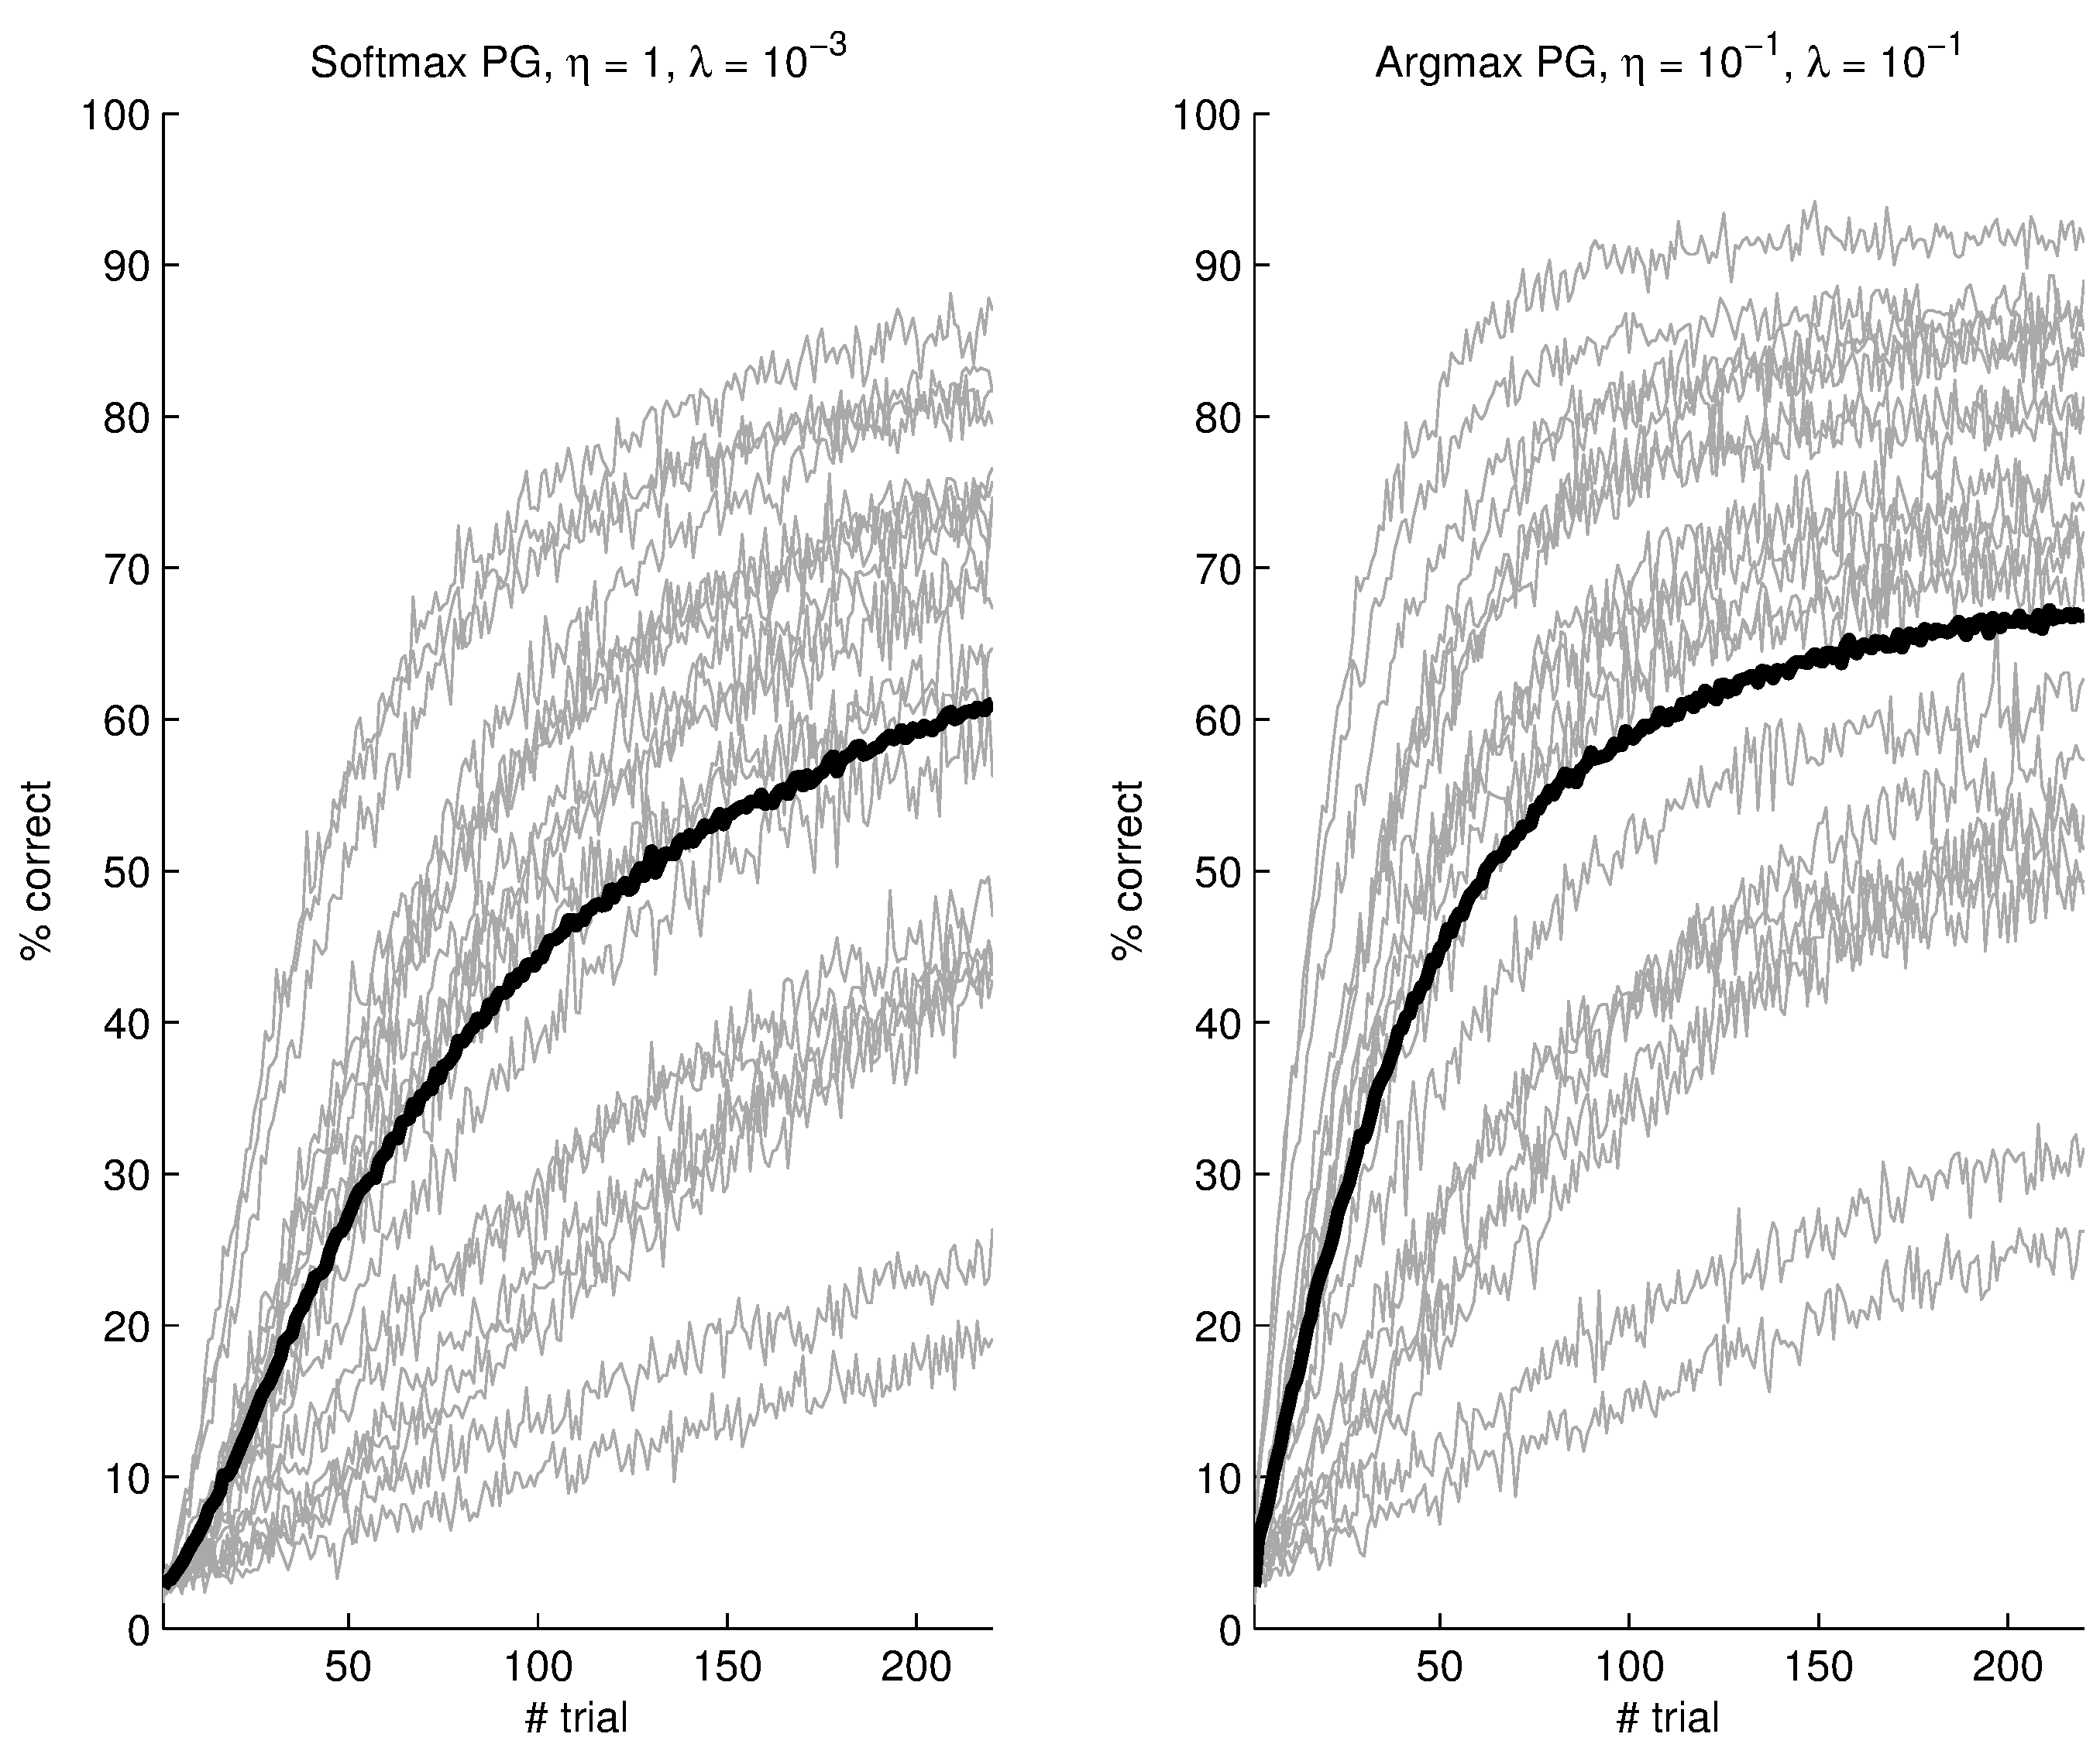
\includegraphics[width=0.7\linewidth]{PG_softmax.png}}
\end{frame}

\begin{frame}\frametitle{XDAWN spatial filter}
	\vspace{-.8cm}
	\cite{Rivet09}
	\centerline{
		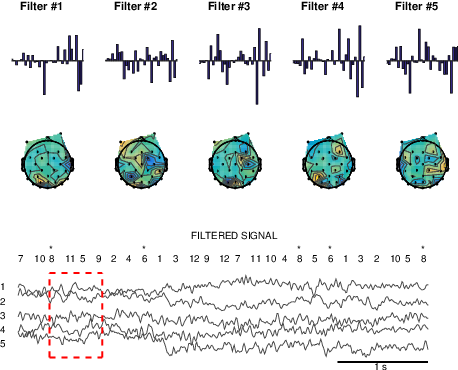
\includegraphics[width=0.7\linewidth]{ijcnn-eeg-filt}
	}
\end{frame}

\begin{frame}\frametitle{Classification improvement after a 25-trials training session}
	%\vspace{-1cm}
\centerline{
	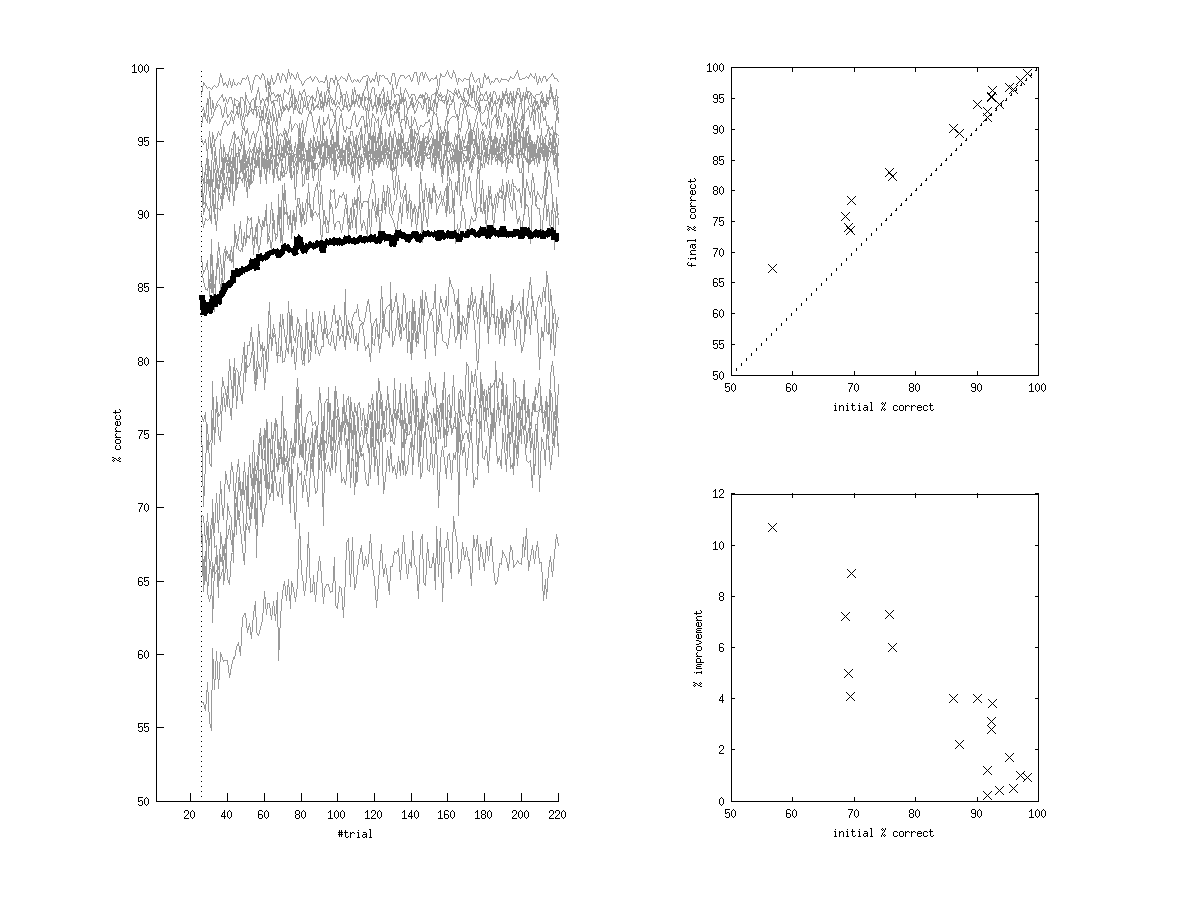
\includegraphics[width=.9\linewidth]{fig_filter_adapt}
}
\end{frame}

\begin{frame}\frametitle{Global recovery after electrode break
		}
	\centerline{
		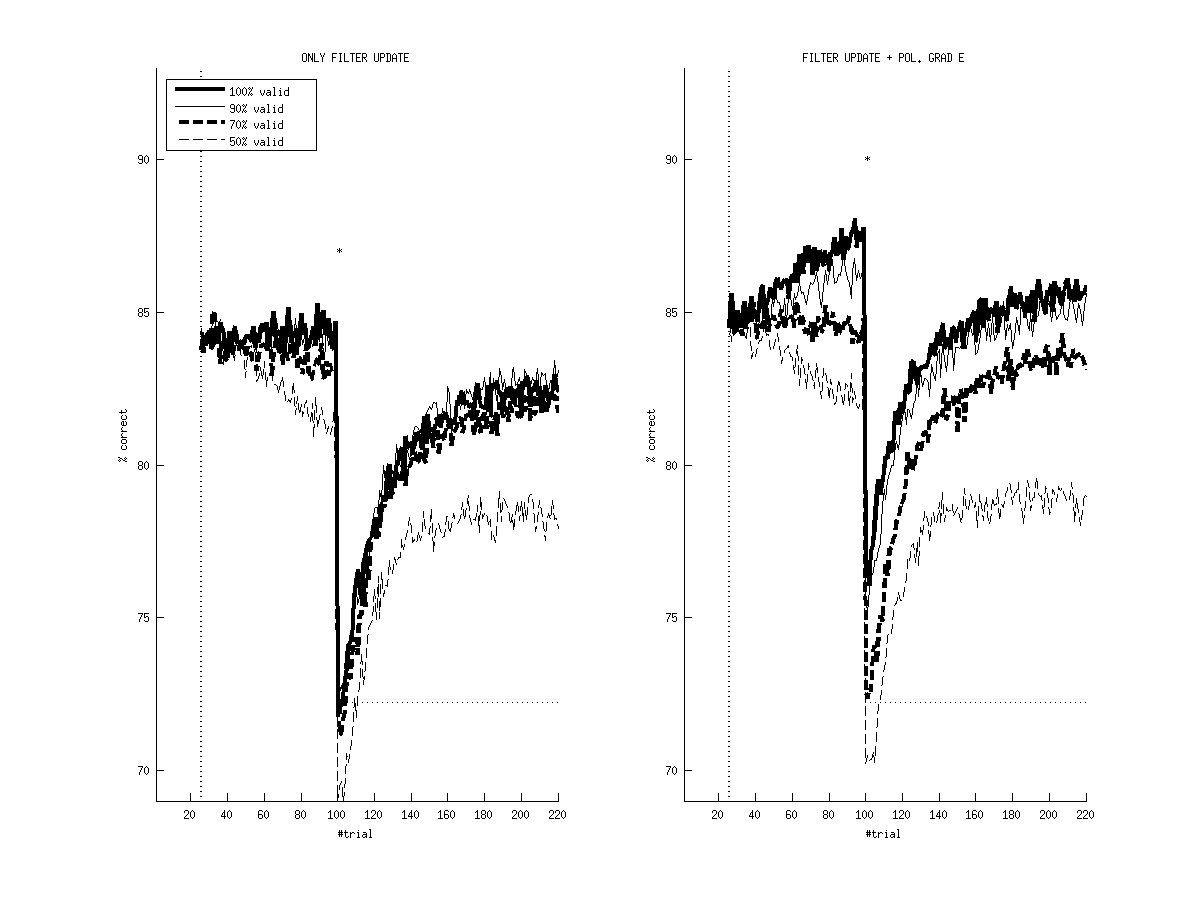
\includegraphics[width=0.9\linewidth]{fig_invalid}
	}
\end{frame}

\begin{frame}\frametitle{Individual recovery, feedback noise = 10\%}
	\centerline{
		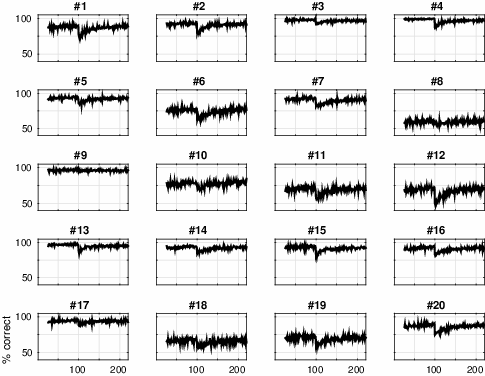
\includegraphics[width=0.7\linewidth]{ijcnn-subj-break-n01}
	}
\end{frame}

\begin{frame}\frametitle{Individual recovery, feedback noise = 30\%}
	\centerline{
		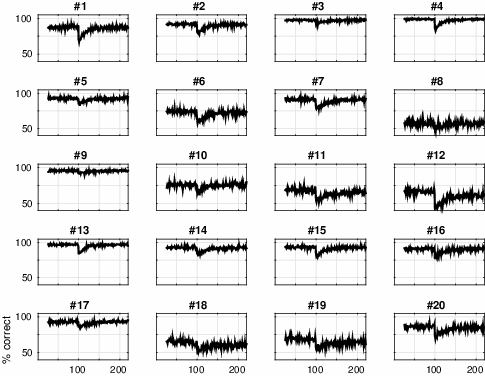
\includegraphics[width=0.7\linewidth]{ijcnn-subj-break-n03}
	}
\end{frame}

\section{Conclusion}
\subsection*{}

\begin{frame}\frametitle{Conclusion}
 \begin{itemize}
  \item  ``Instant'' reward-based policy gradient descent implements classifier training
  \item Binary instant rewards allow non-stochastic exploration (argmax choice instead of softmax) with MLE convergence guaranties 
  \item Regularization allows to track environmental changes
  \item  Is efficient in the P300-speller case, but :
    \begin{itemize}
      \item high variability between subjects
      \item reward extraction problem (difficulty shift)
      \item reward non-reliability bound = 0.7?
    \end{itemize}
 \end{itemize}
\end{frame}

%\begin{frame}{Outlook and discussion}
% \begin{itemize}
%  \item the oddball problem is a specific decision-making problem
%  \begin{itemize}
%    \item ``choose'' the element that fits the best the matching criterions in a set of $K$ candidates
%    \item update the matching criterions
%    \item the candidates are renewed at each trial
%  \end{itemize}
%  \item forgetting (and re-learning) is important in a non-stationary environment:
%  \begin{itemize}
%    \item ($\eta$, $\lambda$) change tracking 
%    \item $\lambda$ regulates the score separation
%    \item $ \frac{1}{\eta\lambda}$ is the sliding window 
%  \end{itemize}
%  \item reward-based learning is efficient in softmax/linear classifiers
%  \begin{itemize}
%  \item bridges between stochastic / probabilistic frameworks
%  \end{itemize}
% \end{itemize}

%\end{frame}



\bibliographystyle{apalike}
\bibliography{biblio-bci}

\end{document}
